
FluiDB is a system that focuses on relational query processing. This
chapter aims to give the reader some idea about where FluiDB fits in
the design space and the historical context in which it was developed.
First we outline a very high level overview of the query language and
operators involved in database management, as well as the the overall
architecture of such systems. Following that we will focus on the
query processing subsystems of relational query databases and some
traditional approaches to query evaluation. Afterwards we will focus
particularly on in-memory relational databases and the tradeoffs that
govern their design. Finally we look into systems that utilize
intermediate result recycling and how they solve the problem of
automatically selecting and maintaining intermediate results for
workloads.

\section{Relational databases}
\label{sec:org5af5e27}
Databases are more than just a method of accessing data. In their
essence they are machines for question answering. The typical database
works in a prepetual loop of reading queries and coming up with
answers based on a set of datapoints. There are two important aspects
that every database needs to define in order to delineate its
operational semantics:

\begin{itemize}
\item The language in which the queries are expressed in
\item The representation of data in terms of which the queries are
expressed and the results are presented.
\end{itemize}

The oldest, most studied and most common model is the relational model
which defines queries in terms of \emph{relational algebra} and organizes
data in \emph{tables} or relations.

A relation is typically an unordered set of tuples
\((d_1,d_2,...,d_k)\) where each element \(d_i\) represents an
attribute. The core relational algebra is an extension of the algabra
of set (that defines operators of set union \(\cup\), intersection
\(\cap\), product \(\times\), and difference \(-\)) that includes the
operators of joins \(\Join\), projection \(\pi\) and selection
\(\sigma\). Upon this foundation relational databases typically define
extra operators to increase the expressive power of the language like
aggregations \(\gamma\), semijoins \(\lsemi\), sorting, limiting, etc.

A typical relational database processes operates in a cascading
fashion. It initially receives a query in textual form. While
relational algebra is the language that underpins the operation of a
relational database it is raraly the language in which users interact
with it. Instead, most relational databases expect queries writen in a
variant of SQL, a query language that is parsed and immediately
translated to a tree of relational algebra operators.

This tree is processed by the query optimizer which rewrites it into a
representation that is efficitent to be executed by taking advantage
of the mathematical properties of RA and often gathered statistics
about the underlying data itself. This process leads to the formation
of a relational algebra expression called the \emph{logical plan}. It is a
high level recipe of what logical operators would produce the
requested result.


Each RA operator is typically implemented by several different
algorithms, each being efficient and even possible in some situations
but not in others. For example a join can be implemented by nested
loops or with merge join.  While the former algorithm is general and
can implement any join, it is very inefficient. On the other hand a
merge join is much more efficient but can only implement joins of the
form \(\Join_{a=b}\) (equijoins). Furhtermore a logical plan typically
contains only implied information about the scheduling of the
operators, for example the logical plan \((\pi A) \Join (\sigma B)\)
implies that the join can not begin being evaluated before the
projection and the selection but the latter can be evaluated in any
order. All these details about the execution of the query are resolved
by the \emph{physical planner}. The physical planner accepts a logical
plan and emits an unambiguous sequence of steps that will produce the
result of the query.

The final step is actually executing the physical plan which is
handled by the \emph{query execution engine}. The execution engine simply
evaluates the physical plan on top of the data, making use of the
correct algorithms, auxiliary structures like indexes managing memory,
handling page-level caching, etc.

\section{Query processing}
\label{sec:org1ddf14b}

Query optimization and more generally query processing and planning
refer to the processes that take place between reading a query and
computing a physical plan. The concerns of query processing are
correcness of the final result and the efficiency of the plan
generated, usually in terms of time, but also in terms of space.

Finding an optimal plan is in the general case NP-complete
\cite{ullmanInformationIntegrationUsing1997}, but query optimizers can
do a good job at finding good plans using heuristics. The selection
and organization of these heuristics as well as query cost estimation
are the main problems that make a query optimizer non-trivial. In
particular there one could separate the the tasks of a query optimizer
into three broad categories:

\begin{itemize}
\item Query rewriting
\item Query plan enumeration
\item Size and cost estimation (cost model)
\end{itemize}

At a very high level the architecture of a query optimizer is
demonstrated in figure \ref{fig:org171f336} and is broadly
comprised of the following components:

\begin{figure}[p]
\centering
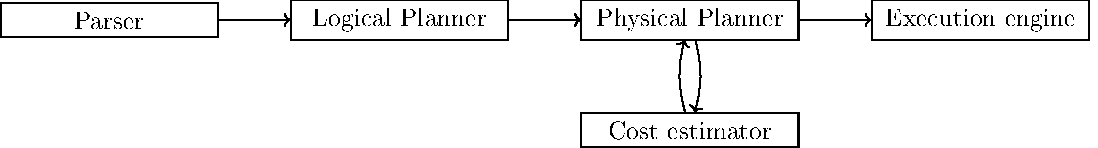
\includegraphics[width=\textwidth]{./imgs/optimizer_architecture.pdf}
\caption{\label{fig:org171f336}Common architecture of a query optimizer.}
\end{figure}

\begin{itemize}
\item The \emph{parser} which receives the query in textual form and produces a
logical plan in the form of an abstract syntax tree.
\item The \emph{deterministic optimizer} or \emph{logical planner} that rewrites the
logical plan applying optimization that are based solely on the
general properties of the relational algebra.
\item The \emph{physical planner} that transforms a logical plan into a
physical plan that can be unambiguously executed by the execution
engine to produce a result. The physical planner typically has at
least some information about the underlying data that the plan will
operate on like estimations about the statistics of the values or
the cardinalities of the relations.
\item The information about the data being manipulated by the plan is
inferred by the \emph{cost estimator}. It uses a cost model to predict
the cost of plans and cardinality of relations by taking into
account the provenance of relations as well as physical properties
of the data like presence of indexes, the data layout, etc.
\end{itemize}

These subsystems are presented here as separate for simplicity and
because in many database systems they are clearly delineated but it is
also common that they blur into each other. For example in some RDBMSs
the physical and logical planner are merged into one
\cite{graefeCascadesFrameworkQuery1995,shankarQueryOptimizationMicrosoft2012,solimanOrcaModularQuery2014}. In
fact, it is more and more common for systems to intersperse query
planning with query execution, adapting the optimization strategy
\cite{graefeDynamicQueryEvaluation1989} to concrete information about
the intermediate results evaluated rather than purely relying on
estimations and predictions
\cite{dingPlanStitchHarnessing2018,chaudhuriPayasyougoFrameworkQuery2008,wuSamplingbasedQueryReoptimization2016,herodotouXplusSqltuningawareQuery2010}. The
degree to which these subsystems are separate is a major concern in
the desgin space of query optimizers.

Another important concern to be considered, and which is indeed is
important in the design of FluiDB, is the number of queries considered
at a time during optimization and the way in which they are
considered. The optimizer usually considers one query at a time and
maintains little or no state between executions. For a very long time,
however muti-query optimization has been researched
\cite{michiardiCachebasedMultiqueryOptimization2021,wangMultiqueryOptimizationMapreduce2013,royEfficientExtensibleAlgorithms2000,rogersMultiqueryOptimization2017}
although no mainstream databases. What is more common in recent years
is recycling intermediate results. These RDBMSs materialize and cache
intermediate relations in the hopes that they will be useful for reuse
in later queries
\cite{perezHistoryawareQueryOptimization2014,nagelRecyclingPipelinedQuery2013,ivanovaArchitectureRecyclingIntermediates2010}.

The final concern that is relevant to the design of FluiDB regards the
traversal and pruning of the search space. As mentioned, query
optimization is generally NP-complete, so the viable options DBMS
designers are left with are randomized algorithms, ML approaches, and
heuristics. Virtually all systems implement heuristics entirely or to
some degree, while more and more incorporate randomized algorithms
\cite{chandeGeneticOptimizationJoin2011} and machine learning
\cite{liMachineLearningDatabases2021,marcusNeoLearnedQuery2019}.

\subsection{Logical and physical query optimization}
\label{sec:org86152ae}

The logical planner accepts a syntax tree in the form of relational
algebra where the operators only contain information about the
semantic meaning of operations and none relating to the algorithms
that will eventually be executed or the input data. It is for all
intents and purposes a rewrite engine for relational algebra. Typical
transformations performed by the logical query optimizer are

\begin{itemize}
\item Predicate normalization to conjunctive normal form, e.g. \((a_0 = 1
  \land a_1 = b_1) \lor b_2 = 3 \hookrightarrow (a_0 = 1 \lor b_2 = 3)
  \land (a_1 = b_1 \lor b_2 = 3)\)
\item Predicate pushdown e.g. \(A \Join_{a_0 = 1 \land p} B
  \hookrightarrow (\sigma_{a_0 = 1} A) \Join_p B\).
\item Cartesian products to joins \(\sigma_p ( A \times B )
  \hookrightarrow A \Join_p B\)
\item Searching the join ordering space.
\end{itemize}

Physical query planner, on the other hand, will specialize the logical
operators deciding on the particular algorithm that should be used. A
physical query planner therefore requires low level information about
the query that relates to indexes available, possible ordering of the
data, materialized views, etc.

Either of the planners needs to enumerate the plans under
consideration while traversing the search space. There are two major
approaches to this:

\begin{itemize}
\item The \emph{top-down} approach, where the planner establishes the top level
operator and branches searching the children, backtracking as
necessary. This was the approach of the decendants of the volcano
\cite{graefeVolcanoOptimizerGenerator1993a} where they implement a
"seach engine" that uses a branch and bound approach to optimization
with caching.
\item The \emph{bottom-up} approach where the builds and connects fragments of
a plan
\cite{raasveldtDuckdbEmbeddableAnalytical2019,kemperHyPerHybridOLTP2011}
\end{itemize}

An important optimizer, on which most modern optimizers are still
being based, is the cascades optimizer
\cite{graefeCascadesFrameworkQuery1995}. In short, cascades keeps track
of \emph{groups} of equivalent expressions of queries and uses those as the
fundamental atom that it manipulates. For example instead of keeping
track of \(A \Join (B \Join C)\) and \((A \Join B) \Join C\)
separately they would be part of the same query group. It then uses a
global hash table (the "memo" structure) to match the best plan that
corresponds to each group.

Many database systems use optimizers similar to cascades (like the
Microsoft SQL server, postgres, and
MemSQL\cite{chenMemSQLQueryOptimizer2016}, and greenplum -- now orca
\cite{solimanOrcaModularQuery2014a} to name a few). Notable among them
is apacha calcite \cite{begoliApacheCalciteFoundational2018}, a
framework for implementing query processing used by a number of
commercial and research databases
\cite{nunesalonsoBuildingPolyglotData2020}.

\subsection{Cost estimation}
\label{sec:org4f8e111}

Probably the hardest aspect of the planner design is the cost
estimation algorithms. These are required in order to select plans a
and to navigate the search space. A good cost model can help basic
planners make decent plans and sophisticated planners make horrible
plans \cite{leisHowGoodAre2015} . As cost estimation we refer to a
number of different related procedures that are broadly the estimation
of the cost of an arbitrary plan and include the prediction of the
cardinality of not yet materialized relations.

It seems that the most important challenges involved in the design of
a cost model is that we are fundamentally operating with scares with
scarce and highly uncertain information. Especially relating to
cardinality estimation, the most important of the tasks involved,
uncertainty and bad predictions propagate and make make it extremely
hard for the planers to make correct decisions. Consider for example a
join. Some joins are similar to cartesian products, producing large
output tables, and some joins are more similar to lookups producing
only a few rows. A cost model that confuses the kind of join will make
very bad predictions w.r.t. the cost of any relational algebra
expression that uses said join. Therefore join order estimation, that
is a critical aspect of planning.

Cost estimation is beyond the scope of FluiDB and we only implement
the most naive cardinality estimation but it is worth mentioning how
more mature systems approach the issue. Cardinality estimation most
commonly takes the form of selectivity estimation, i.e. what
percentage of tuples from the input make it to the output of a
selection or a join. This is sensitive to the statistical
properties of the values and the selection/join predicates.

The most common approach to this issue is to maintain pre-computed
statistics relating to the primary tables. This is much better than
keeping no stats but they are very hard to maintain and their
effectiveness becomes very limited for complex queries. Another
approach employed is to delay the decisions of the optimizer and
essentially merge the panner with the execution engine. This does not
completely eliminate the problem but it allows the system to have more
up to date and precise data that would allow it to correct cource
early in the event of exceptionally bad estimations. One family of
techniques that is becoming popular and was initially used in IBM DB2
\cite{stillgerLEODB2LearningOptimizer2001}, is caching the statistics
of previously computed relations and use that data to make better
predictions in the future. More recently this takes the form of
employing machine learning to learn from past cardinalities
\cite{ortizEmpiricalAnalysisDeep2019}.

To give the reader a more well rounded intuition of the state of cost
estimation besides cardinality estimation it is worth mentioning that,
to estimate the cost of an operatior, postgres uses magic configurable
variables to weigh IO with CPU evaluation time, while DB2 runs
microbenchmarks on the production system to make these estimations.


\section{in-memory relational databases}
\label{sec:org96af629}
In-memory databases are databases where all the data lives in main
memory. The design of in-memory databases is different from the desgn
of a disk-backed database in a number of respects. To name a few:

\begin{itemize}
\item Page buffers have no use and caching of data in general has very
different goals. While in disk databases caches are mainly used to
avoid disk IO, in memory databases they focus on short-circuiting
computation.
\item Concurrency control is much simpler as storage synchronization
concerns are almost entirely eliminated.
\item In disk backed databases only a small percentage of time is spend on
actual computation \cite{harizopoulosOLTPLookingGlass2018}. Much of
the non-compute latency is directly linked to the persintent
storage.
\end{itemize}

On the other hand there are concerns that are specific to the lack of
backing database storage. A few of those are:

\begin{itemize}
\item Should the system rely on record IDs like in a persistent database
or can it use direct pointers to records?
\item Error prone software can bring the data to an irrecoverable state.
\item Query execution algorithms have fundamentally different
charadteristics. While in persistent databases IO dominates the
runtime the bottlenecks for an in-memory database are much more
complex and they can include things like locking, cache misses,
predicate evaluation data movements.
\item As main memory is a much less abundant resourse than presistent
storage, in-memory databases are often distributed making network a
major concern.
\end{itemize}

One increasingly common technique to address many of these issues,
which is also used by FluiDB, is \textbf{code generation}. Since workloads
for in-memory databases are typically CPU bound, there are major gains
in performance to be had by specializing the code being executed. The
typical generic code being run makes heavy use of virtual function
calls and conditionals inside tight loops which kills performance on
virtually all modern architectures. The value proposition of code
generation is to inline or hardcode the virtual functions and erase
the conditionals at runtime to reduce the number of operations and
make better use of hardware optimizations.

We identify 4 different approaches in the literature to solving this
problem:

\subsection{Transpilation}
\label{sec:orgbf8a953}

Transpilation of a physical plan to a systems language like C or C++
which is then fed to an off the shelf compiler
\cite{krikellasGeneratingCodeHolistic2010}. This approach is expensive
but it generates highly efficient code more easily debuggable
execution plans. The most notable complete database system that used
this technique is Microsoft Hekaton that generates C code and some
older versions of MemSQL. For FluiDB we reuse a lot of techiques
introduced in HIQUE \cite{krikellasGeneratingCodeHolistic2010} to
translate physical plans to template-heavy C++ code, making the
assumption that query compilation will be much faster than the query
runtime.

\subsection{Thrid party compilers}
\label{sec:orgdf395cd}

JIT compilation has received a lot of attention in the compiler
community, especially in the context of the JVM. A number of database
systems have taken advantage of this to speed up query execution. Most
notable of these are SPARK \cite{armbrustSparkSQLRelational2015}, which
generates scala AST which is then converted to JVM byte code, and
Neo4j that directly generates bytecode out of the queries.

Systems like Peloton \cite{menonRelaxedOperatorFusion2017} and recently
postgres \cite{sharyginQueryCompilationPostgreSQL2017} compile query
plans to LLVM IR code that is then fed to the LLVM compiler to
generate high performance machine code. Notable among the systems that
use this approach is HyPer \cite{neumannEvolutionCompilingQueryEngine}
which addresses the problem of the query compilation overhead with an
adaptive execution apprach: they built an IR interpreter that starts
running the query while the compiler does proper compilation of the
LLVM IR program being interpreted. Cheap queries are thus completed
reasonably fast while in the case of complex queries the interpreted
program is seamlessly replaced by the compiled one once the LLVM
compiler finishes generating machine code.

\subsection{Direct machine code generation}
\label{sec:org344a12c}

Some databases do not reuse any compiler or JIT-ing VM, but rather
directly generate highly specific machine code out of the physical
plan. The first system to attempt that, like most techniques used
today, was System R which originally compiled SQL statements directly
to machine code by stitching together code fragments from a fragment
library \cite{chamberlinHistoryEvaluationSystem1981} but it was quickly
deprecated due to the large engineering effort required. Oracle [ref]
also includes similar to some of their databases and MemSQL express
their plans in a custom language called MPL (MemSQL Plan Language) for
which they have a custom compiler that translates it directly to
machine code.

\subsection{Custom execution engines}
\label{sec:org7bca3a3}

TODO: read these papers a bit more carefully

A final category is per-database code generation rather than per-query
code generation. Volcano/EXODUS
\cite{graefeVolcanoOptimizerGenerator1993a} and more recently SageDB
\cite{kraskaSageDBLearnedDatabase} generate the optimizer and execution
engine that is specific to the database schema but not to the queries.


\section{Intermediate result recycling}
\label{sec:org1a32ec6}
A materialized view is a relation defined by a query that is
persistently stored. A view that is not stored is said to be
virtual. \textbf{View selection} is the process of selecting an apropritate
set of materialized views to imporve the performance of a workload
\cite{mamiSurveyViewSelection2012}.  Automated materialized view
selection or intermediate view recycling has been on the radar of the
database research community for a while now. A few approaches to this
problem have to do with AND/OR directed acyclic graphs
\cite{guptaSelectionViewsMaterialize1997}, modeling the problem as a
state optimization \cite{theodoratosDataWarehouseConfiguration1997},
and lattices to represent data cube operations (i.e. multiple
aggregations over the same relation) \cite{ImplementingDataCubes}.

A related problem is multi-query optimization
\cite{theodoratosDataWarehouseConfiguration1997} that attempts to plan
multiple queries simultaneously. An efficient solution using AND/OR
DAGs was proposed by Roy in \cite{royEfficientExtensibleAlgorithms2000}
where they insert queries and their subqueries in a graph and attempt
to evaluate a plan by traversing that graph from multiple sources in a
fashion similar to volcano optimization. Building on that Kathuria
et. al. prresent an approximation algorithm that runs in time
quadratic to the number of common subexpressions and provides
theoretical guarantees on the quality of the solution obtained
\cite{kathuriaEfficientProvableMultiquery2017}.

Researchers have further looked at opportunistically reusing
intermediate results that would be materialized
\cite{ivanovaArchitectureRecyclingIntermediates2010,nagelRecyclingPipelinedQuery2013}. It
has been researched in non-strictly database contexts like MapReduce
\cite{elghandourReStoreReusingResults2012a}, and there have been
attempts to unify the planner with the materialized view selection
engine \cite{perezHistoryawareQueryOptimization2014a}. Notable in this
field is Nectar \cite{gundaNectarAutomaticManagement2010} which is also
not an RDBMs. It automatically compresses rarely used data into
programs that generate that data. Nectar focuses on sharing
computation and data as much as possible.

Work such as MRShare \cite{nykielMRShareSharingMultiple2010} tries to
bridge the gap betweem intermediate result recycling and MQO by
automatically grouping queries in a workload in such a way that
computation can be maximally shared.
